% Options for packages loaded elsewhere
\PassOptionsToPackage{unicode}{hyperref}
\PassOptionsToPackage{hyphens}{url}
\PassOptionsToPackage{dvipsnames,svgnames,x11names}{xcolor}
%
\documentclass[
  letterpaper,
  DIV=11,
  numbers=noendperiod]{scrartcl}

\usepackage{amsmath,amssymb}
\usepackage{iftex}
\ifPDFTeX
  \usepackage[T1]{fontenc}
  \usepackage[utf8]{inputenc}
  \usepackage{textcomp} % provide euro and other symbols
\else % if luatex or xetex
  \usepackage{unicode-math}
  \defaultfontfeatures{Scale=MatchLowercase}
  \defaultfontfeatures[\rmfamily]{Ligatures=TeX,Scale=1}
\fi
\usepackage{lmodern}
\ifPDFTeX\else  
    % xetex/luatex font selection
\fi
% Use upquote if available, for straight quotes in verbatim environments
\IfFileExists{upquote.sty}{\usepackage{upquote}}{}
\IfFileExists{microtype.sty}{% use microtype if available
  \usepackage[]{microtype}
  \UseMicrotypeSet[protrusion]{basicmath} % disable protrusion for tt fonts
}{}
\makeatletter
\@ifundefined{KOMAClassName}{% if non-KOMA class
  \IfFileExists{parskip.sty}{%
    \usepackage{parskip}
  }{% else
    \setlength{\parindent}{0pt}
    \setlength{\parskip}{6pt plus 2pt minus 1pt}}
}{% if KOMA class
  \KOMAoptions{parskip=half}}
\makeatother
\usepackage{xcolor}
\setlength{\emergencystretch}{3em} % prevent overfull lines
\setcounter{secnumdepth}{-\maxdimen} % remove section numbering
% Make \paragraph and \subparagraph free-standing
\makeatletter
\ifx\paragraph\undefined\else
  \let\oldparagraph\paragraph
  \renewcommand{\paragraph}{
    \@ifstar
      \xxxParagraphStar
      \xxxParagraphNoStar
  }
  \newcommand{\xxxParagraphStar}[1]{\oldparagraph*{#1}\mbox{}}
  \newcommand{\xxxParagraphNoStar}[1]{\oldparagraph{#1}\mbox{}}
\fi
\ifx\subparagraph\undefined\else
  \let\oldsubparagraph\subparagraph
  \renewcommand{\subparagraph}{
    \@ifstar
      \xxxSubParagraphStar
      \xxxSubParagraphNoStar
  }
  \newcommand{\xxxSubParagraphStar}[1]{\oldsubparagraph*{#1}\mbox{}}
  \newcommand{\xxxSubParagraphNoStar}[1]{\oldsubparagraph{#1}\mbox{}}
\fi
\makeatother


\providecommand{\tightlist}{%
  \setlength{\itemsep}{0pt}\setlength{\parskip}{0pt}}\usepackage{longtable,booktabs,array}
\usepackage{calc} % for calculating minipage widths
% Correct order of tables after \paragraph or \subparagraph
\usepackage{etoolbox}
\makeatletter
\patchcmd\longtable{\par}{\if@noskipsec\mbox{}\fi\par}{}{}
\makeatother
% Allow footnotes in longtable head/foot
\IfFileExists{footnotehyper.sty}{\usepackage{footnotehyper}}{\usepackage{footnote}}
\makesavenoteenv{longtable}
\usepackage{graphicx}
\makeatletter
\def\maxwidth{\ifdim\Gin@nat@width>\linewidth\linewidth\else\Gin@nat@width\fi}
\def\maxheight{\ifdim\Gin@nat@height>\textheight\textheight\else\Gin@nat@height\fi}
\makeatother
% Scale images if necessary, so that they will not overflow the page
% margins by default, and it is still possible to overwrite the defaults
% using explicit options in \includegraphics[width, height, ...]{}
\setkeys{Gin}{width=\maxwidth,height=\maxheight,keepaspectratio}
% Set default figure placement to htbp
\makeatletter
\def\fps@figure{htbp}
\makeatother
% definitions for citeproc citations
\NewDocumentCommand\citeproctext{}{}
\NewDocumentCommand\citeproc{mm}{%
  \begingroup\def\citeproctext{#2}\cite{#1}\endgroup}
\makeatletter
 % allow citations to break across lines
 \let\@cite@ofmt\@firstofone
 % avoid brackets around text for \cite:
 \def\@biblabel#1{}
 \def\@cite#1#2{{#1\if@tempswa , #2\fi}}
\makeatother
\newlength{\cslhangindent}
\setlength{\cslhangindent}{1.5em}
\newlength{\csllabelwidth}
\setlength{\csllabelwidth}{3em}
\newenvironment{CSLReferences}[2] % #1 hanging-indent, #2 entry-spacing
 {\begin{list}{}{%
  \setlength{\itemindent}{0pt}
  \setlength{\leftmargin}{0pt}
  \setlength{\parsep}{0pt}
  % turn on hanging indent if param 1 is 1
  \ifodd #1
   \setlength{\leftmargin}{\cslhangindent}
   \setlength{\itemindent}{-1\cslhangindent}
  \fi
  % set entry spacing
  \setlength{\itemsep}{#2\baselineskip}}}
 {\end{list}}
\usepackage{calc}
\newcommand{\CSLBlock}[1]{\hfill\break\parbox[t]{\linewidth}{\strut\ignorespaces#1\strut}}
\newcommand{\CSLLeftMargin}[1]{\parbox[t]{\csllabelwidth}{\strut#1\strut}}
\newcommand{\CSLRightInline}[1]{\parbox[t]{\linewidth - \csllabelwidth}{\strut#1\strut}}
\newcommand{\CSLIndent}[1]{\hspace{\cslhangindent}#1}

\KOMAoption{captions}{tableheading}
\makeatletter
\@ifpackageloaded{caption}{}{\usepackage{caption}}
\AtBeginDocument{%
\ifdefined\contentsname
  \renewcommand*\contentsname{Table of contents}
\else
  \newcommand\contentsname{Table of contents}
\fi
\ifdefined\listfigurename
  \renewcommand*\listfigurename{List of Figures}
\else
  \newcommand\listfigurename{List of Figures}
\fi
\ifdefined\listtablename
  \renewcommand*\listtablename{List of Tables}
\else
  \newcommand\listtablename{List of Tables}
\fi
\ifdefined\figurename
  \renewcommand*\figurename{Figure}
\else
  \newcommand\figurename{Figure}
\fi
\ifdefined\tablename
  \renewcommand*\tablename{Table}
\else
  \newcommand\tablename{Table}
\fi
}
\@ifpackageloaded{float}{}{\usepackage{float}}
\floatstyle{ruled}
\@ifundefined{c@chapter}{\newfloat{codelisting}{h}{lop}}{\newfloat{codelisting}{h}{lop}[chapter]}
\floatname{codelisting}{Listing}
\newcommand*\listoflistings{\listof{codelisting}{List of Listings}}
\makeatother
\makeatletter
\makeatother
\makeatletter
\@ifpackageloaded{caption}{}{\usepackage{caption}}
\@ifpackageloaded{subcaption}{}{\usepackage{subcaption}}
\makeatother

\ifLuaTeX
  \usepackage{selnolig}  % disable illegal ligatures
\fi
\usepackage{bookmark}

\IfFileExists{xurl.sty}{\usepackage{xurl}}{} % add URL line breaks if available
\urlstyle{same} % disable monospaced font for URLs
\hypersetup{
  pdftitle={Maternal Health Risk Prediction},
  pdfauthor={Mengen Liu, Roy Oh, Kim Tan Palanca, \& Nicolas Zhu},
  colorlinks=true,
  linkcolor={blue},
  filecolor={Maroon},
  citecolor={Blue},
  urlcolor={Blue},
  pdfcreator={LaTeX via pandoc}}


\title{Maternal Health Risk Prediction}
\usepackage{etoolbox}
\makeatletter
\providecommand{\subtitle}[1]{% add subtitle to \maketitle
  \apptocmd{\@title}{\par {\large #1 \par}}{}{}
}
\makeatother
\subtitle{A Comparative Study of Machine Learning Model Performance}
\author{Mengen Liu, Roy Oh, Kim Tan Palanca, \& Nicolas Zhu}
\date{}

\begin{document}
\maketitle


\section{Summary}\label{summary}

This project aims to use machine learning to predict maternal health
risk based on key physiological factors by comparing the performances
between two models. Maternal health are a major concern in healthcare.
Hence, early risk assessment is crucial for the welfare of both the
mother and child. By leveraging structured data from the Maternal Health
Risk Dataset, we trained and evaluated machine learning models to
classify maternal health risk levels into three different classes: low,
mid, and high risk.

The dataset contains 1,014 records with features such as age, blood
pressures, blood sugar levels, body temperature and heart rate. Our goal
will be to determine whether machine learning algorithms could
accurately predict risk levels based on these physiological markers. We
will first conduct an exploratory data analysis before building any of
the models. Once we have trained the models, their accuracies will be
evaluated as measures of performance.

\section{Introduction}\label{introduction}

Maternal health can be defined as ``the health condition of women during
preganancy, childbirth, and the postnatal period (WHO 2025). This is a
critical area of healthcare, as complications during preganancy and
childbirth can lead to severe consequences for both mothers and
newborns. According to the (WHO 2024), around 800 women died each day in
2020 due to preventable causes related to maternal health, further
emphasizing the need for risk assessment measures.

Historically, risk assessment have been carried out by medical
professionals that relied heavily on clinical expertise and constant
monitoring. However, traditional approaches to monitoring basic
physiological indicators often lacked efficiency in identifying
potential complications (Mu, Yan, and Zhu 2023). Since the boom of
machine learning (ML), many members of the academe have explored the use
of ML in maternal health risk prediction, offering data-driven
approaches to enhance early detection and intervention to offload the
burden on overworked medical professionals (Bajaj, Kumari, and Bansal
2023; Mu, Yan, and Zhu 2023; Ukrit et al. 2024).

The analysis will utilize the
\href{https://archive.ics.uci.edu/dataset/863/maternal+health+risk}{Maternal
Health Risk} dataset sourced from the UC Irvine Machine Learning
Repository (Ahmed 2020). Consisting of 1014 observations, this dataset
includes the following 7 features:

\begin{itemize}
\tightlist
\item
  \texttt{Age}: Age of the patient (in years).
\item
  \texttt{SystolicBP}: Systolic Blood Pressure (mmHg).
\item
  \texttt{DiastolicBP}: Diastolic Blood Pressure (mmHg).
\item
  \texttt{BS\ (Blood\ Sugar\ Level)}: Blood sugar concentration
  (mmol/L).
\item
  \texttt{BodyTemp}: Body temperature (°F).
\item
  \texttt{HeartRate}: Heart rate (beats per minute).
\item
  \texttt{RiskLevel}: The target variable, categorized into low risk,
  mid risk, and high risk.
\end{itemize}

\subsection{Project Question}\label{project-question}

To contribute to this discourse, this research aims to conduct a
comparative study on the performance of two ML techniques in predicting
maternal health risk, assessing each model's reliability in identifying
risk levels. The following research question guides this analysis:

\begin{itemize}
\tightlist
\item
  \emph{Which machine learning model most accurately predicts the
  maternal health risk level (low, medium, or high risk) based on
  physiological indicators such as blood sugar levels, body temperature,
  and other relevant health factors?}
\end{itemize}

\section{Methods}\label{methods}

For this analysis, the data will first be loaded into the notebook then
cleaned to handle any possible missing values and ensure its usability
for the various models. Following the data cleaning stabe will be an
exploratory data analysis (EDA) to gain a comprehensive view of the
data. This step will include visualizing the summary statistics,
distributions, and correlations between variables to determine any
patterns in the data prior to the model development.

This study will implement 3 ML classification models:

\begin{enumerate}
\def\labelenumi{\arabic{enumi}.}
\tightlist
\item
  Baseline (Majority Class)
\item
  Logistic Regression
\item
  Random Forest
\end{enumerate}

Each model will be evaluated based on the appropriate classification
metric to compare their relative performance in maternal health risk
prediction.

\subsection{Wrangling and Cleaning the
Data}\label{wrangling-and-cleaning-the-data}

From Table~\ref{tbl-missing-vals}, we find that there are no missing
values in the dataset.

\begin{table}

\caption{\label{tbl-missing-vals}Check for Missing Values}

\centering{

\begin{verbatim}
# A tibble: 7 x 2
  feature        na
  <chr>       <dbl>
1 Age             0
2 SystolicBP      0
3 DiastolicBP     0
4 BS              0
5 BodyTemp        0
6 HeartRate       0
7 RiskLevel       0
\end{verbatim}

}

\end{table}%

Furthermore, we find that the features \texttt{Age},
\texttt{SystolicBP}, \texttt{DiastolicBP}, \texttt{BS},
\texttt{BodyTemp}, and \texttt{HeartRate} are numeric variables, while
\texttt{RiskLevel} is currently a character variable. Moreover,
Table~\ref{tbl-risk-levels} shows that there are three categories under
\texttt{RiskLevel}: high risk, mid risk, and low risk. Given the three
distinct categories under the target feature, we will modify
\texttt{RiskLevel} to a factor variable to appropriately reflect its
categorical nature in further analysis.

\begin{table}

\caption{\label{tbl-risk-levels}Distinct Risk Levels}

\centering{

\begin{verbatim}
# A tibble: 3 x 1
  RiskLevel
  <chr>    
1 high risk
2 low risk 
3 mid risk 
\end{verbatim}

}

\end{table}%

Table~\ref{tbl-clean} shows a snapshot of the cleaned data.

\begin{table}

\caption{\label{tbl-clean}Sample of the Cleaned Data}

\centering{

\begin{verbatim}
# A tibble: 6 x 7
    Age SystolicBP DiastolicBP    BS BodyTemp HeartRate RiskLevel
  <dbl>      <dbl>       <dbl> <dbl>    <dbl>     <dbl> <chr>    
1    25        130          80 15          98        86 high risk
2    35        140          90 13          98        70 high risk
3    29         90          70  8         100        80 high risk
4    30        140          85  7          98        70 high risk
5    35        120          60  6.1        98        76 low risk 
6    23        140          80  7.01       98        70 high risk
\end{verbatim}

}

\end{table}%

\subsection{Exploratory Data Analysis}\label{exploratory-data-analysis}

\subsubsection{Summary Statistics}\label{summary-statistics}

\begin{table}

\caption{\label{tbl-summ-stats}Summary Statistics}

\centering{

\begin{verbatim}
# A tibble: 6 x 6
  Feature       min   max   mean median    sd
  <chr>       <dbl> <dbl>  <dbl>  <dbl> <dbl>
1 Age            10    70  29.9    26   13.5 
2 SystolicBP     70   160 113.    120   18.4 
3 DiastolicBP    49   100  76.5    80   13.9 
4 BS              6    19   8.73    7.5  3.29
5 BodyTemp       98   103  98.7    98    1.37
6 HeartRate       7    90  74.3    76    8.09
\end{verbatim}

}

\end{table}%

\subsubsection{Age Distributions}\label{age-distributions}

Since age is an important factor in maternal health, we visualize the
age distribution by risk level. From the visualization, high risk
individuals have a higher median age around 35 years old. Additionally,
the interquartile range indicates that the high risk group has more
variation in age. We observe some outliers in the low and mid risk
groups. Based on the visualization, older aged individuals seem more
associated with maternal health risks.

\begin{figure}

\centering{

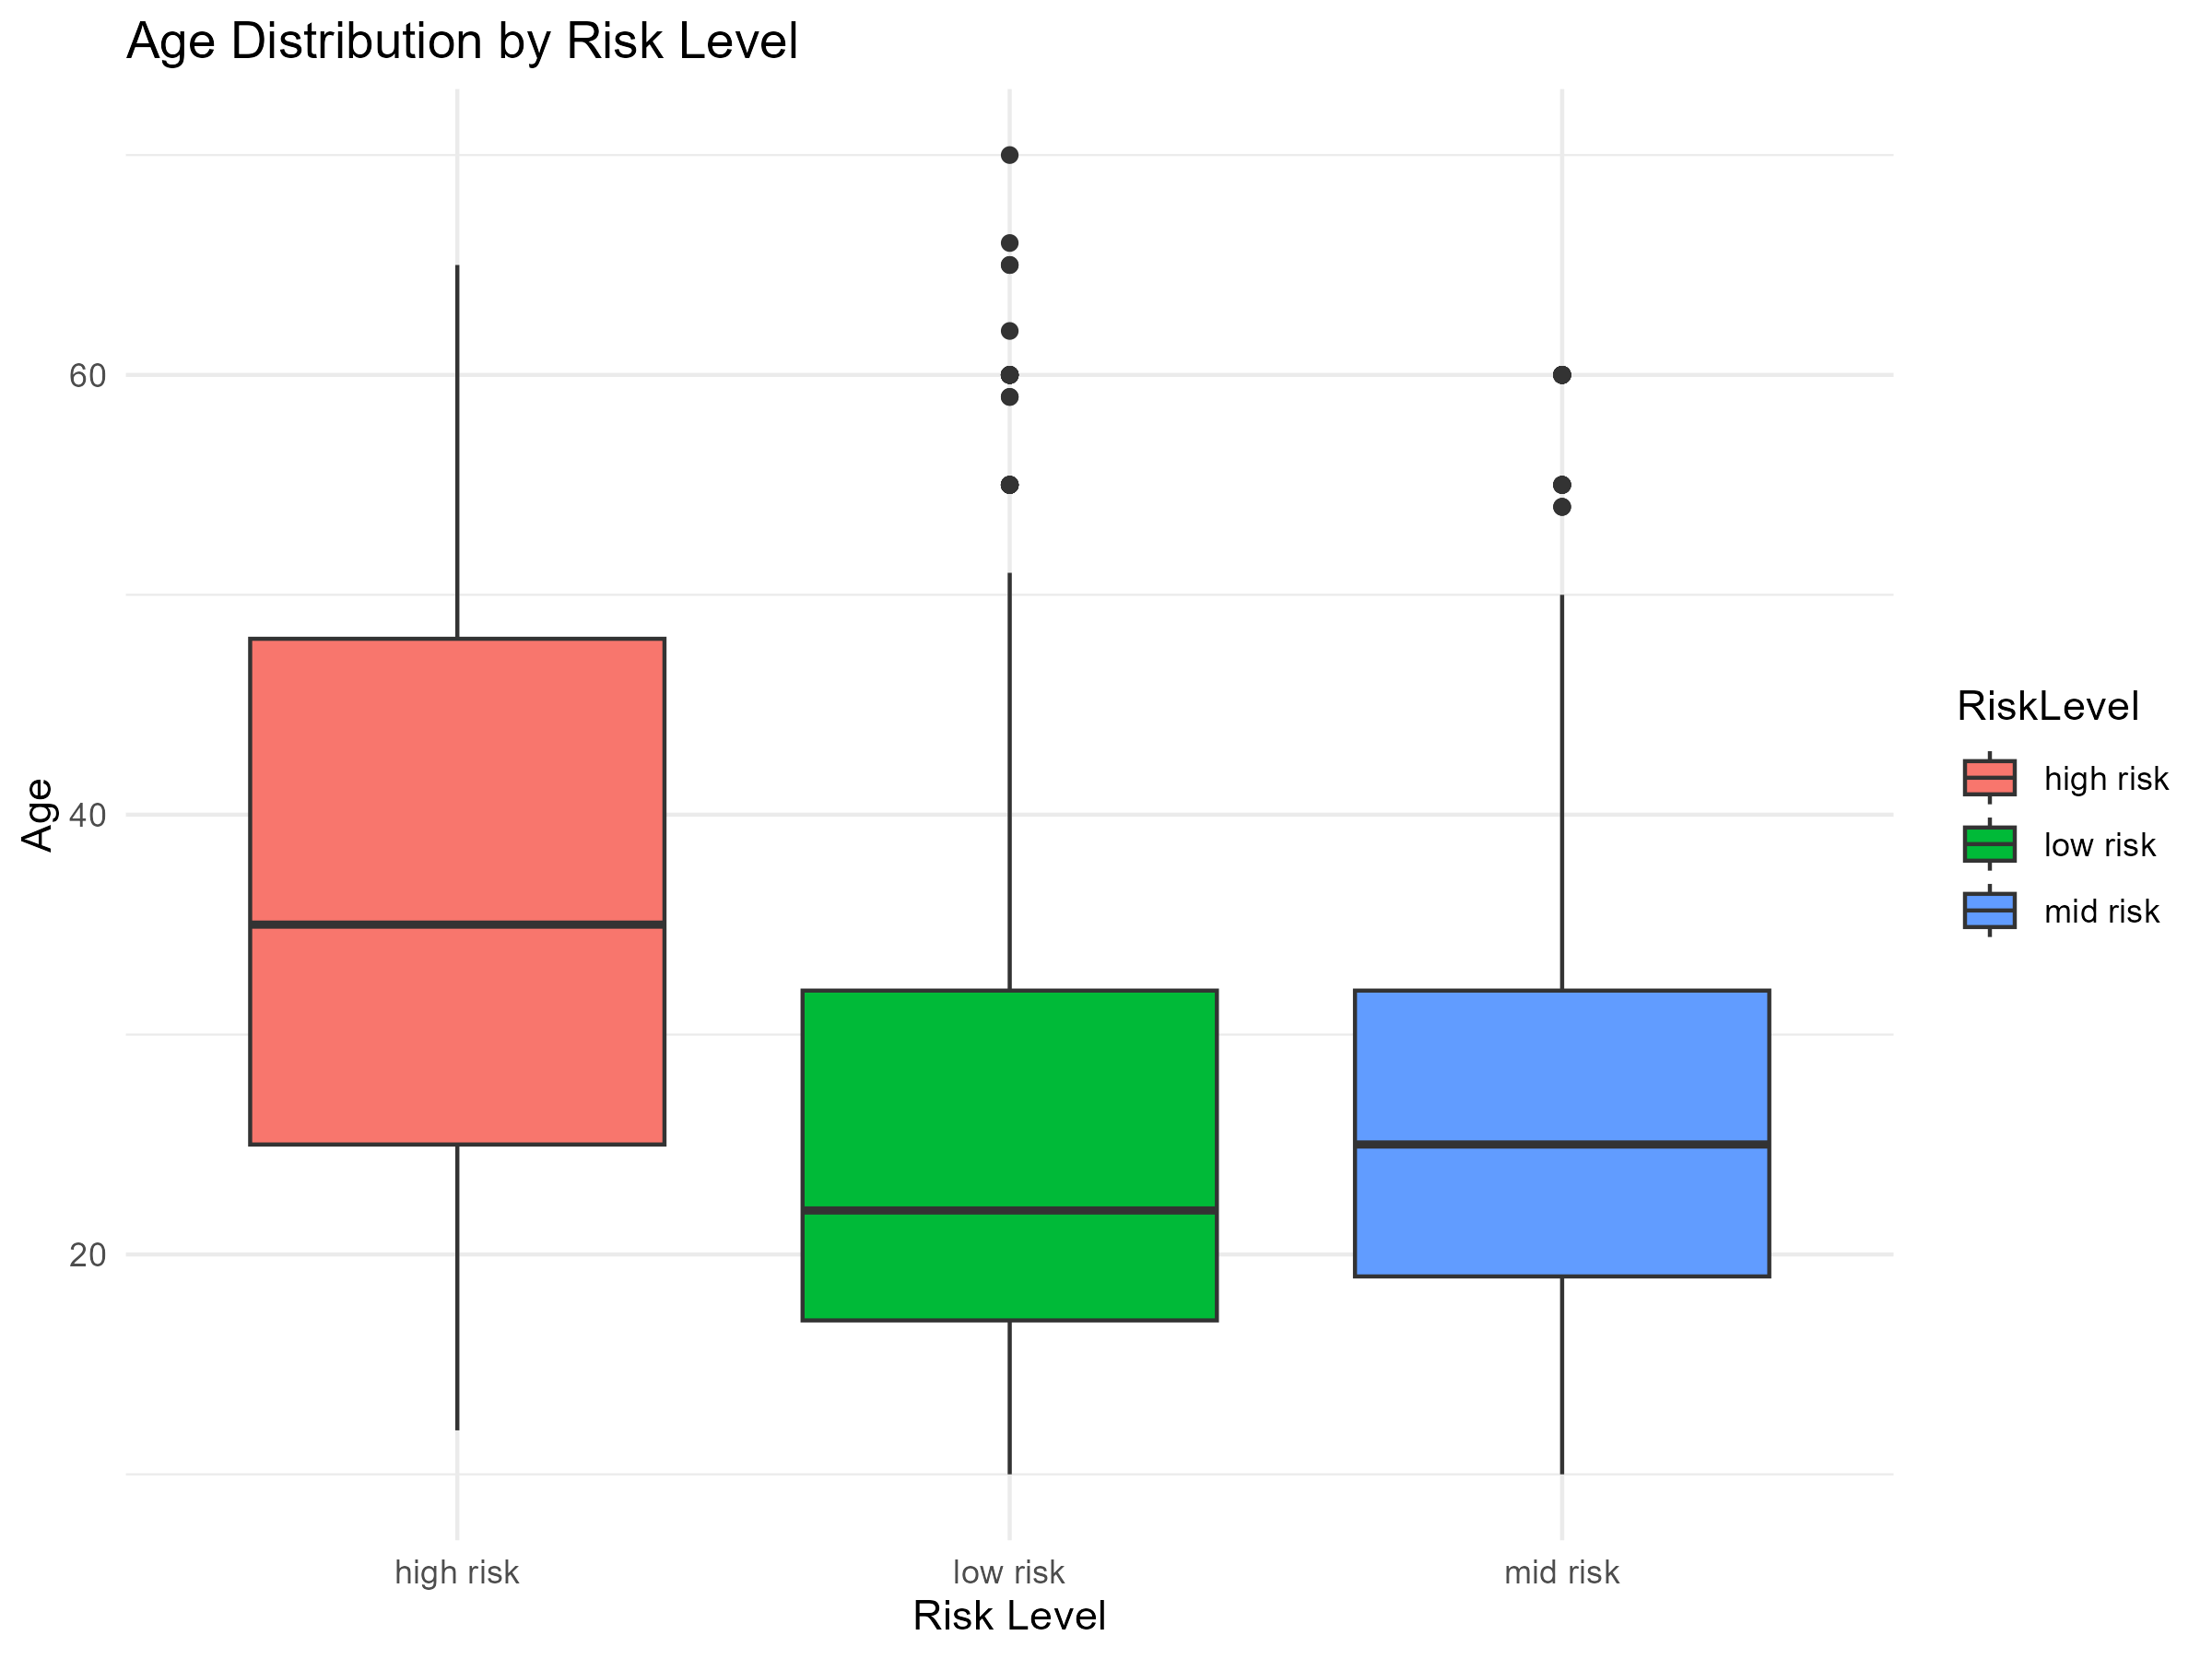
\includegraphics{../outputs/images/age_distribution.png}

}

\caption{\label{fig-age-distrib}Age Distribution by Risk Level}

\end{figure}%

Since the target classes seem relatively balanced, it would be
appropriate to use \textbf{accuracy} as the main scoring metric.
Accuracy is given by the number correct prediction out of all
predictions made

\subsubsection{Correlation Matrix}\label{correlation-matrix}

\begin{figure}

\begin{minipage}{0.50\linewidth}

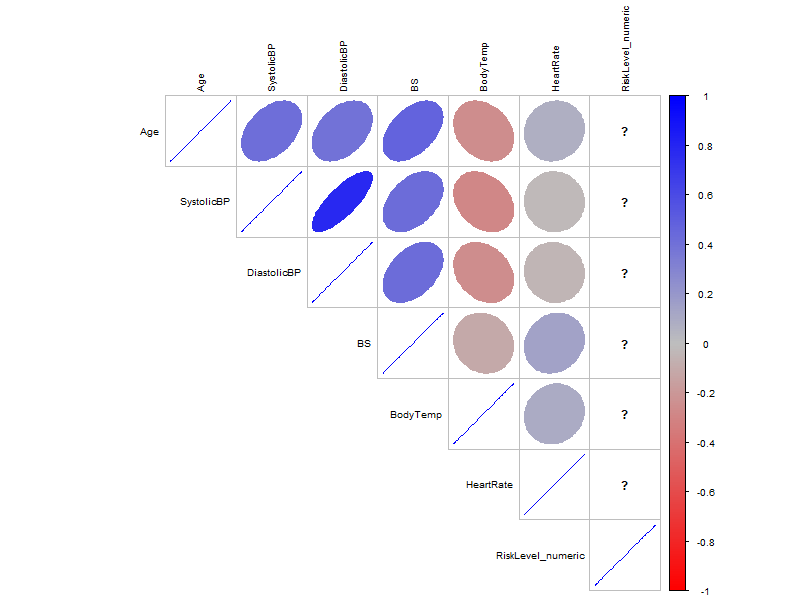
\includegraphics{../outputs/images/correlation_matrix.png}

\subcaption{\label{}Ellipse Correlation}
\end{minipage}%
%
\begin{minipage}{0.50\linewidth}

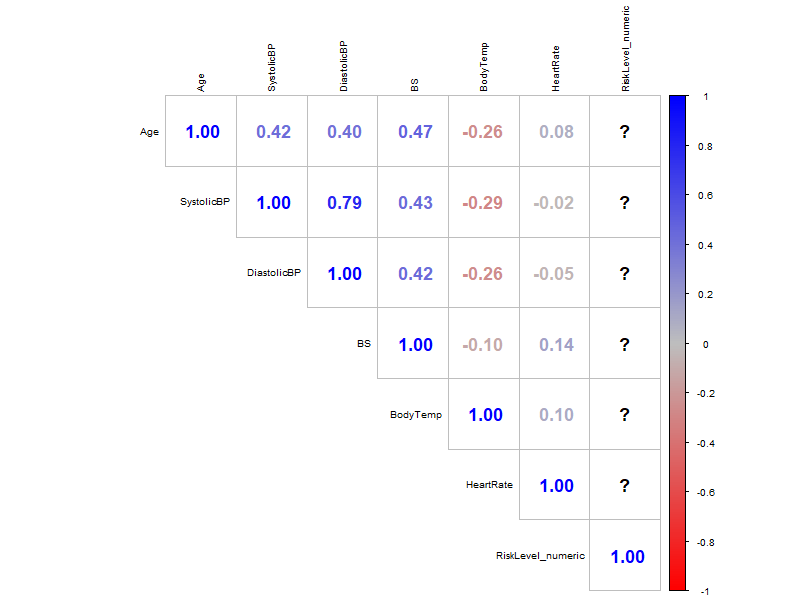
\includegraphics{../outputs/images/correlation_values.png}

\subcaption{\label{}Correlation Values}
\end{minipage}%

\caption{\label{fig-corr-mat}Correlation Matrix}

\end{figure}%

All of the variables have a positive correlation with RiskLevel,
indicating that increases in these variables generally correspond to a
higher maternal health risk. BS (Blood Sugar level) has the strongest
correlation of 0.7870065, suggesting it is likely to be the most
influential factor. We thought age would have a stronger correlation
with RiskLevel, however, systolic blood pressure and diastolic blood
pressure seems to have a stronger correlation with RiskLevel than age.
Additionally, there are no signs of concern for multicollinearity issues
in this dataset.

These findings may be a possible reason for the outliers observed above.
Younger individuals with high blood pressures or sugar levels may be
classified into higher risk levels. This indicates the importance of
other factors.

\section{Classification Model
Building}\label{classification-model-building}

\subsection{Train/Test Splitting}\label{traintest-splitting}

The cleaned data will be split into training and testing sets, with 80\%
allocated for training and 20\% for testing.

\subsection{Baseline Model (Majority
Class)}\label{baseline-model-majority-class}

The baseline model has shown an accuracy of 0.4009901.

\subsection{Multinomial Logistic
Regression}\label{multinomial-logistic-regression}

The MLR model is as follows:

\begin{table}

\caption{\label{tbl-mlr-coefs}Multinomial Logistic Regression Model}

\centering{

\begin{verbatim}
Call:
multinom(formula = RiskLevel ~ ., data = train_data)

Coefficients:
          (Intercept)          Age SystolicBP DiastolicBP        BS  BodyTemp
mid risk    -48.31965 -0.007544419 0.05929424 -0.03362508 0.3747446 0.3986736
high risk   -95.40388 -0.023851313 0.06420403  0.02026145 0.7873117 0.7628112
           HeartRate
mid risk  0.03010820
high risk 0.06461374

Residual Deviance: 1246.411 
AIC: 1274.411 
\end{verbatim}

}

\end{table}%

\begin{table}

\caption{\label{tbl-mlr-log-odds}Exponentiated coefficients to transform
log-odds to odds ratio}

\centering{

\begin{verbatim}
# A tibble: 14 x 6
   y.level   term        estimate std.error   statistic   p.value
   <chr>     <chr>          <dbl>     <dbl>       <dbl>     <dbl>
 1 mid risk  (Intercept) 1.04e-21  0.000176 -274453.    0        
 2 mid risk  Age         9.92e- 1  0.00774       -0.975 3.29e-  1
 3 mid risk  SystolicBP  1.06e+ 0  0.00813        7.30  2.98e- 13
 4 mid risk  DiastolicBP 9.67e- 1  0.0106        -3.18  1.48e-  3
 5 mid risk  BS          1.45e+ 0  0.0870         4.31  1.67e-  5
 6 mid risk  BodyTemp    1.49e+ 0  0.0130        30.6   2.72e-205
 7 mid risk  HeartRate   1.03e+ 0  0.0124         2.43  1.50e-  2
 8 high risk (Intercept) 3.69e-42  0.000147 -650390.    0        
 9 high risk Age         9.76e- 1  0.0123        -1.95  5.16e-  2
10 high risk SystolicBP  1.07e+ 0  0.0121         5.31  1.12e-  7
11 high risk DiastolicBP 1.02e+ 0  0.0153         1.32  1.86e-  1
12 high risk BS          2.20e+ 0  0.0929         8.48  2.32e- 17
13 high risk BodyTemp    2.14e+ 0  0.0172        44.3   0        
14 high risk HeartRate   1.07e+ 0  0.0167         3.87  1.10e-  4
\end{verbatim}

}

\end{table}%

\subsubsection{Model Testing}\label{model-testing}

\begin{table}

\caption{\label{tbl-mlr-predict}Multinomial Logistic Regression
Predicted Probabilities}

\centering{

\begin{verbatim}
# A tibble: 202 x 5
      ID Predicted_Class `low risk` `mid risk` `high risk`
   <dbl> <chr>                <dbl>      <dbl>       <dbl>
 1     1 high risk           0.0131      0.204     0.783  
 2     2 low risk            0.483       0.364     0.153  
 3     3 mid risk            0.257       0.636     0.107  
 4     4 low risk            0.509       0.402     0.0892 
 5     5 low risk            0.652       0.249     0.0990 
 6     6 low risk            0.893       0.103     0.00394
 7     7 mid risk            0.326       0.596     0.0778 
 8     8 low risk            0.626       0.315     0.0595 
 9     9 low risk            0.664       0.203     0.133  
10    10 low risk            0.818       0.149     0.0333 
# i 192 more rows
\end{verbatim}

}

\end{table}%

The multinomial logistic regression has only given us an slightly better
accuracy than the baseline with a score of 0.6138614.

Lastly, we plot multinomial logistic regression graphs to visualize how
predicted probabilities changes among different variable levels.

\begin{figure}

\centering{

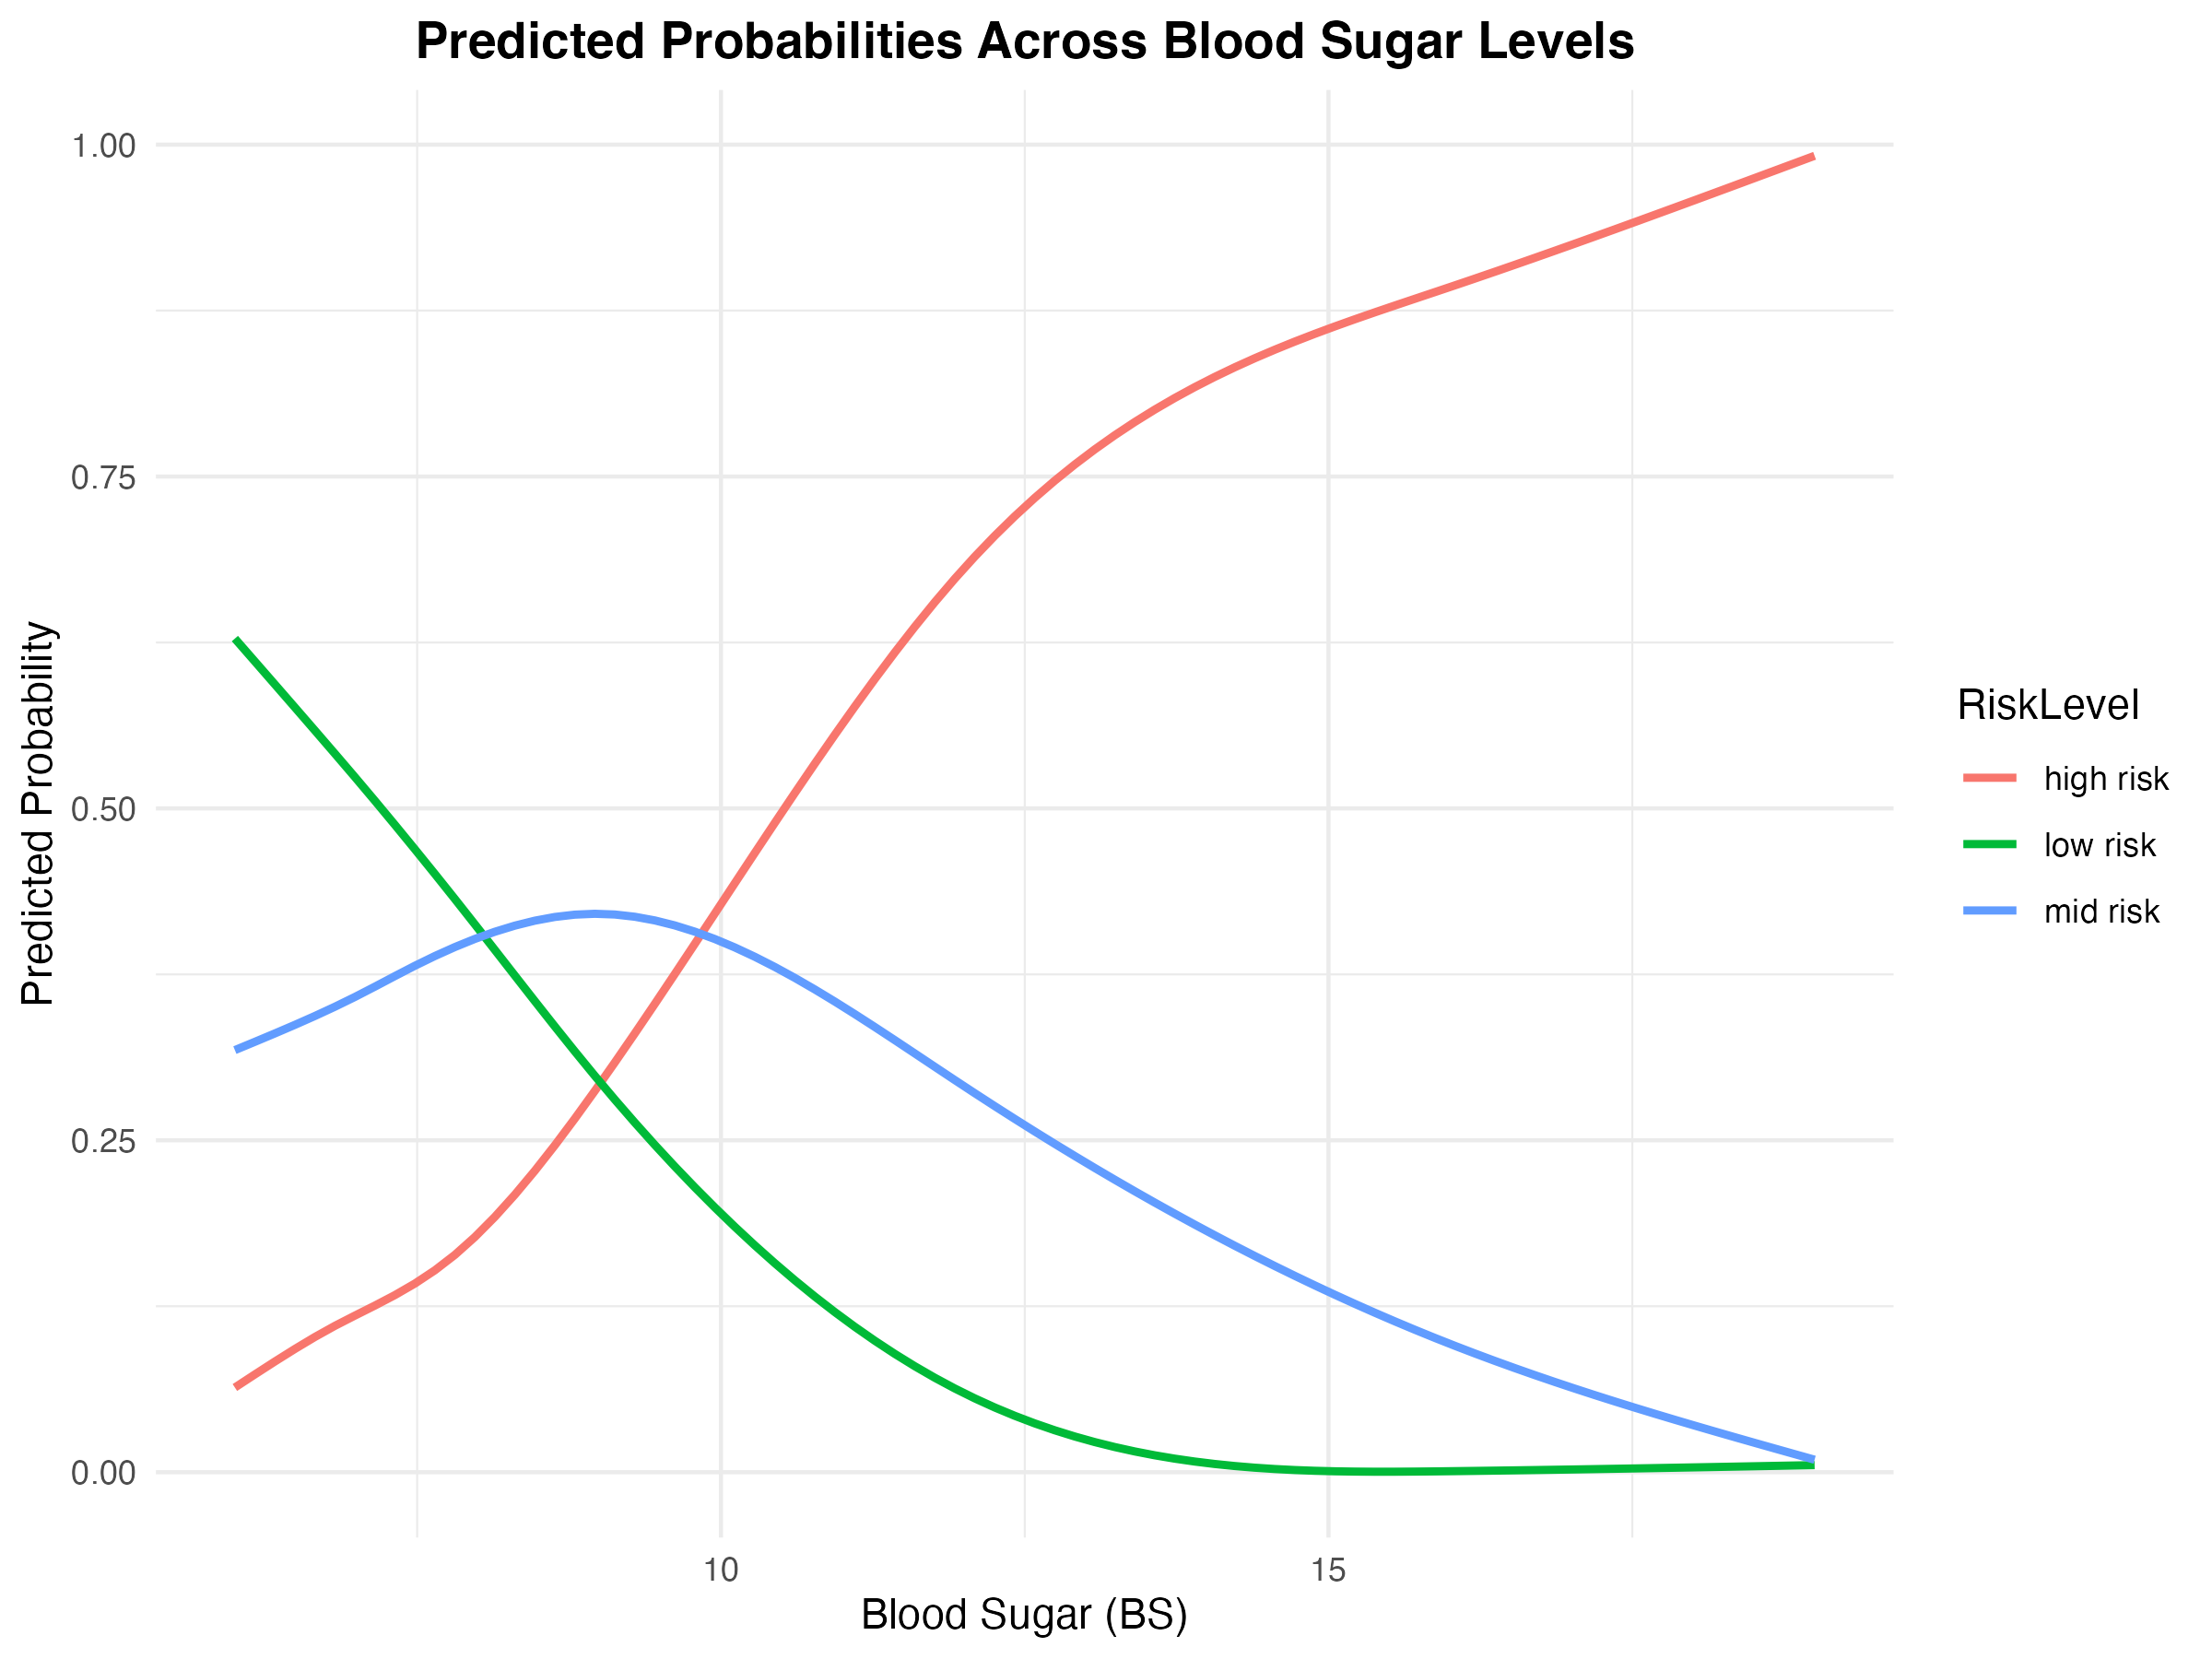
\includegraphics[width=0.7\textwidth,height=\textheight]{../outputs/images/blood_sugar_plot.png}

}

\caption{\label{fig-blood-sugar}Predicted Probabilities Across Blood
Sugar Levels}

\end{figure}%

We observe from Figure~\ref{fig-blood-sugar} that as blood sugar level
rises the probability of high risk increases, while mid and low risk
decreases.

\subsection{Random Forest}\label{random-forest}

The random forest model is as follows:

\begin{table}

\caption{\label{tbl-rf}Random Forest Model}

\centering{

\begin{verbatim}

Call:
 randomForest(formula = RiskLevel ~ ., data = train_data, ntree = 500,      importance = TRUE) 
               Type of random forest: classification
                     Number of trees: 500
No. of variables tried at each split: 2

        OOB estimate of  error rate: 18.84%
Confusion matrix:
          high risk low risk mid risk class.error
high risk       193       11       14   0.1146789
low risk          7      264       54   0.1876923
mid risk         21       46      202   0.2490706
\end{verbatim}

}

\end{table}%

Here are the parameters that have been passed through the randomForest
object:

\begin{itemize}
\tightlist
\item
  \texttt{RiskLevel\ \textasciitilde{}\ .}: Predicts RiskLevel based on
  all other features
\item
  \texttt{ntree\ =\ 500}: Uses 500 trees in the forest
\item
  \texttt{importance} = TRUE: Computes feature importance
\end{itemize}

\subsubsection{Model Testing}\label{model-testing-1}

Now that the model is trained using our train set, we can make
predictions on the test set. We find that the random forest model
provides a better accuracy score than the multinomial regression model
with an accuracy of 0.8811881. Moreover, we can assess feature
importances with a random forest model.

\begin{figure}

\centering{

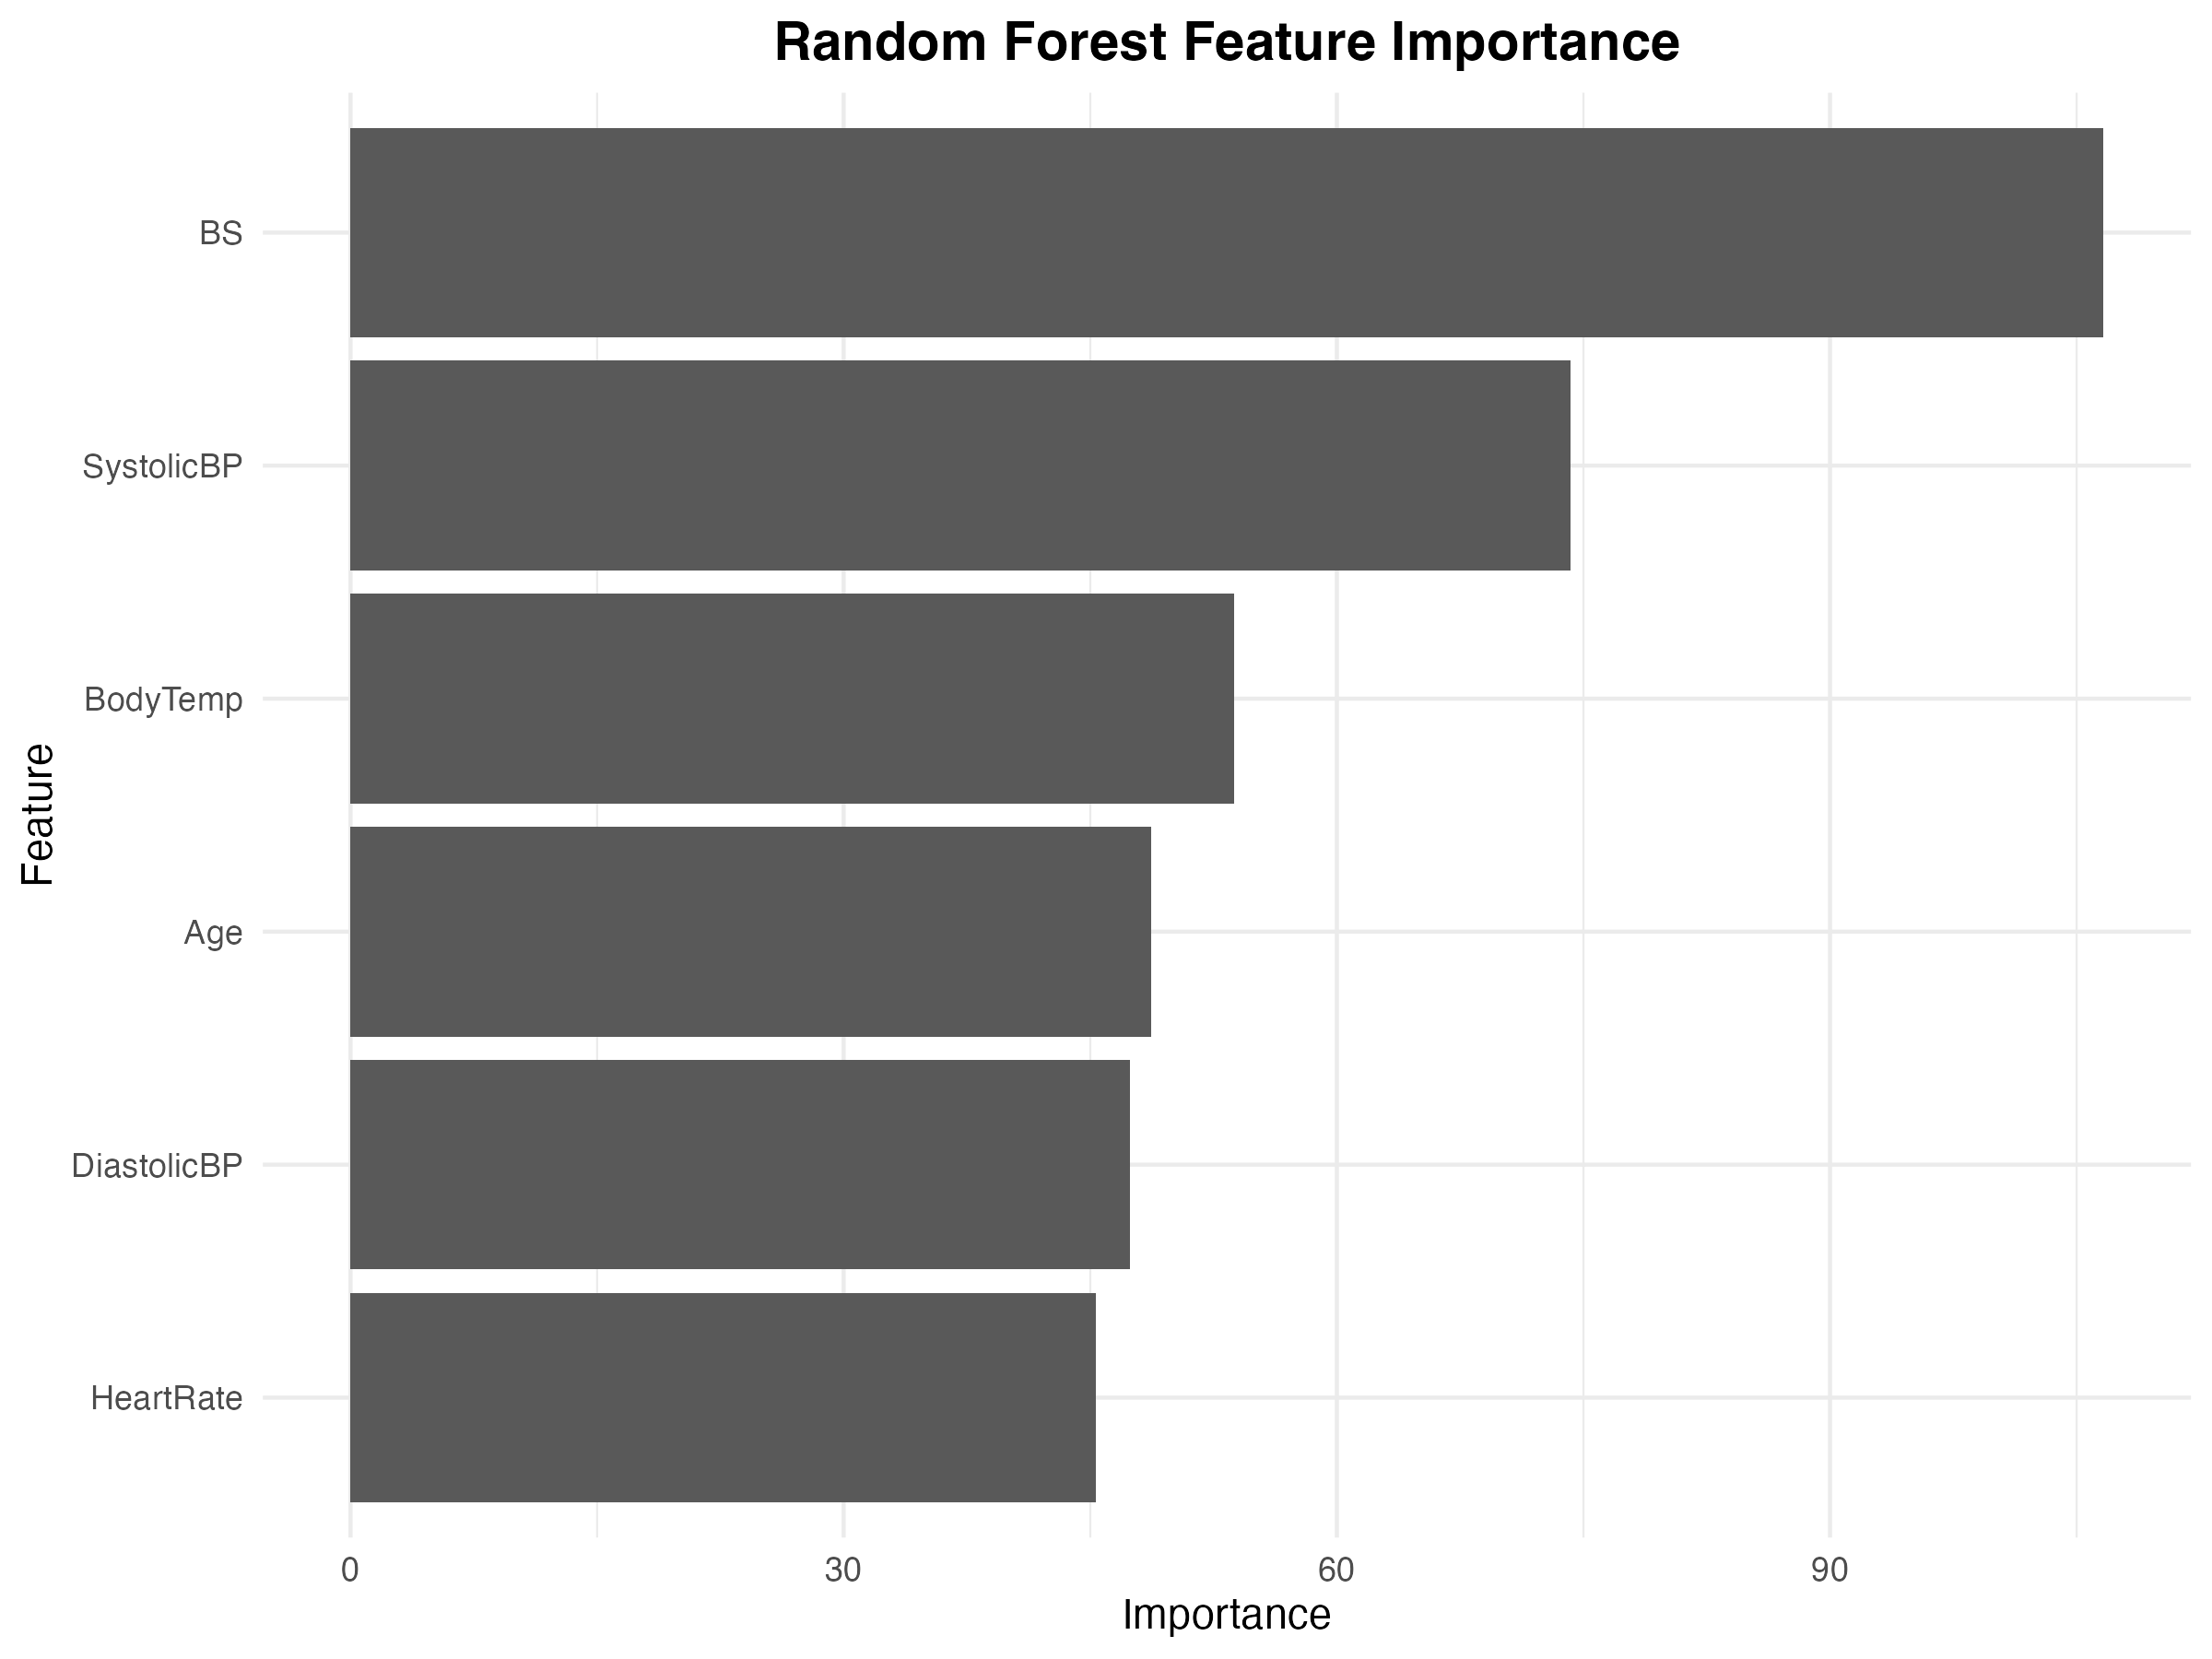
\includegraphics[width=0.7\textwidth,height=\textheight]{../outputs/images/rf_feature_importance.png}

}

\caption{\label{fig-rf-feat-importance}Random Forest Feature
Importances}

\end{figure}%

Based on Figure~\ref{fig-rf-feat-importance} above, we see that the
model identifies blood sugar, systolic blood pressure, and body
temperature as the top predictors of maternal health risk (i.e., have
the most predictive power). With blood sugar specifically, we see that
it's feature importance reaches over 100 indicating that it is highly
influential in predicting maternal health risk compared to the other
features.

\section{Results}\label{results}

\begin{table}

\caption{\label{tbl-base-conf-mat}Baseline Confusion Matrix}

\centering{

\begin{verbatim}
# A tibble: 9 x 4
  True      Predicted Frequency Percentage
  <chr>     <chr>         <dbl>      <dbl>
1 high risk high risk         0       NA  
2 low risk  high risk        54       26.7
3 mid risk  high risk         0       NA  
4 high risk low risk          0       NA  
5 low risk  low risk         81       40.1
6 mid risk  low risk          0       NA  
7 high risk mid risk          0       NA  
8 low risk  mid risk         67       33.2
9 mid risk  mid risk          0       NA  
\end{verbatim}

}

\end{table}%

\begin{table}

\caption{\label{tbl-mlr-conf-mat}Multinomial Logistic Regression
Confusion Matrix}

\centering{

\begin{verbatim}
# A tibble: 9 x 4
  True      Predicted Frequency Percentage
  <chr>     <chr>         <dbl>      <dbl>
1 high risk high risk        38       76  
2 low risk  high risk         2        2.1
3 mid risk  high risk        14       25.5
4 high risk low risk          2        4  
5 low risk  low risk         62       63.9
6 mid risk  low risk         17       30.9
7 high risk mid risk         10       20  
8 low risk  mid risk         33       34  
9 mid risk  mid risk         24       43.6
\end{verbatim}

}

\end{table}%

\begin{table}

\caption{\label{tbl-rf-conf-mat}Random Forest Confusion Matrix}

\centering{

\begin{verbatim}
# A tibble: 9 x 4
  True      Predicted Frequency Percentage
  <chr>     <chr>         <dbl>      <dbl>
1 high risk high risk        52       92.9
2 low risk  high risk         1        1.1
3 mid risk  high risk         1        1.7
4 high risk low risk          1        1.8
5 low risk  low risk         74       85.1
6 mid risk  low risk          6       10.2
7 high risk mid risk          3        5.4
8 low risk  mid risk         12       13.8
9 mid risk  mid risk         52       88.1
\end{verbatim}

}

\end{table}%

\subsection{Comparison of Results}\label{comparison-of-results}

\begin{figure}

\centering{

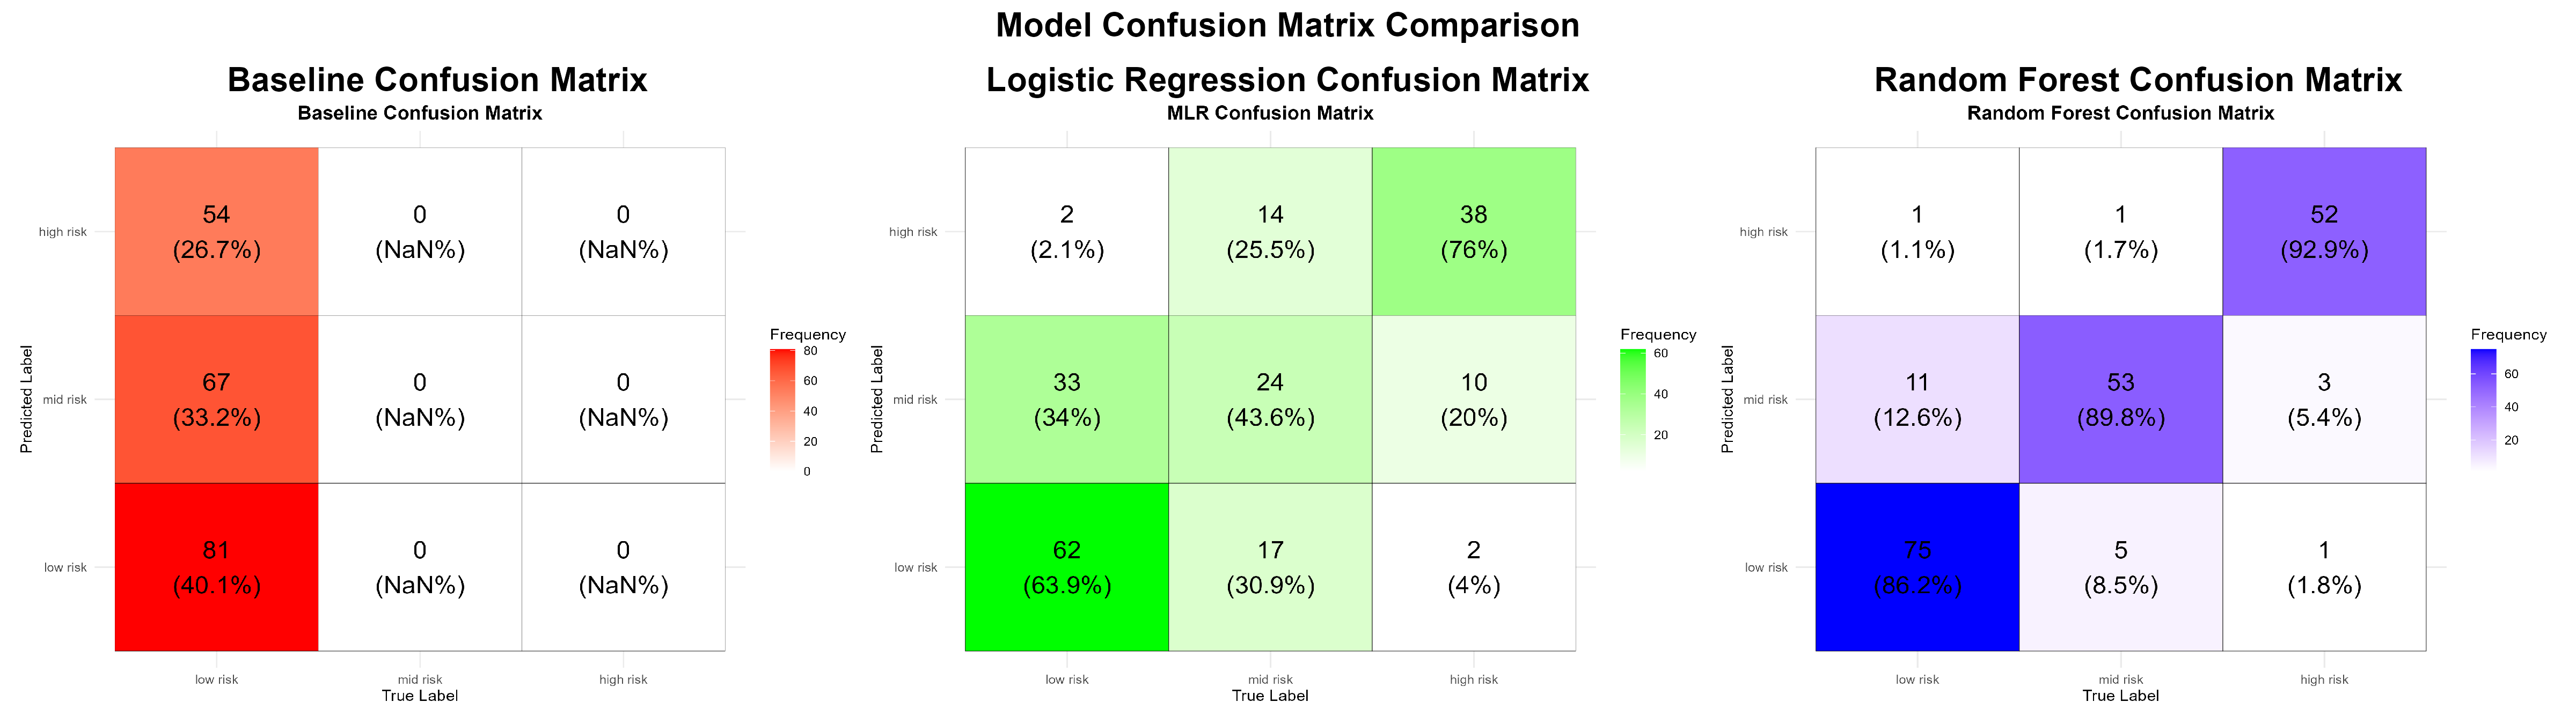
\includegraphics{../outputs/images/conf_matrix_comparison.png}

}

\caption{\label{fig-conf-comparison}ML Model Confusion Matrices}

\end{figure}%

\begin{figure}

\centering{

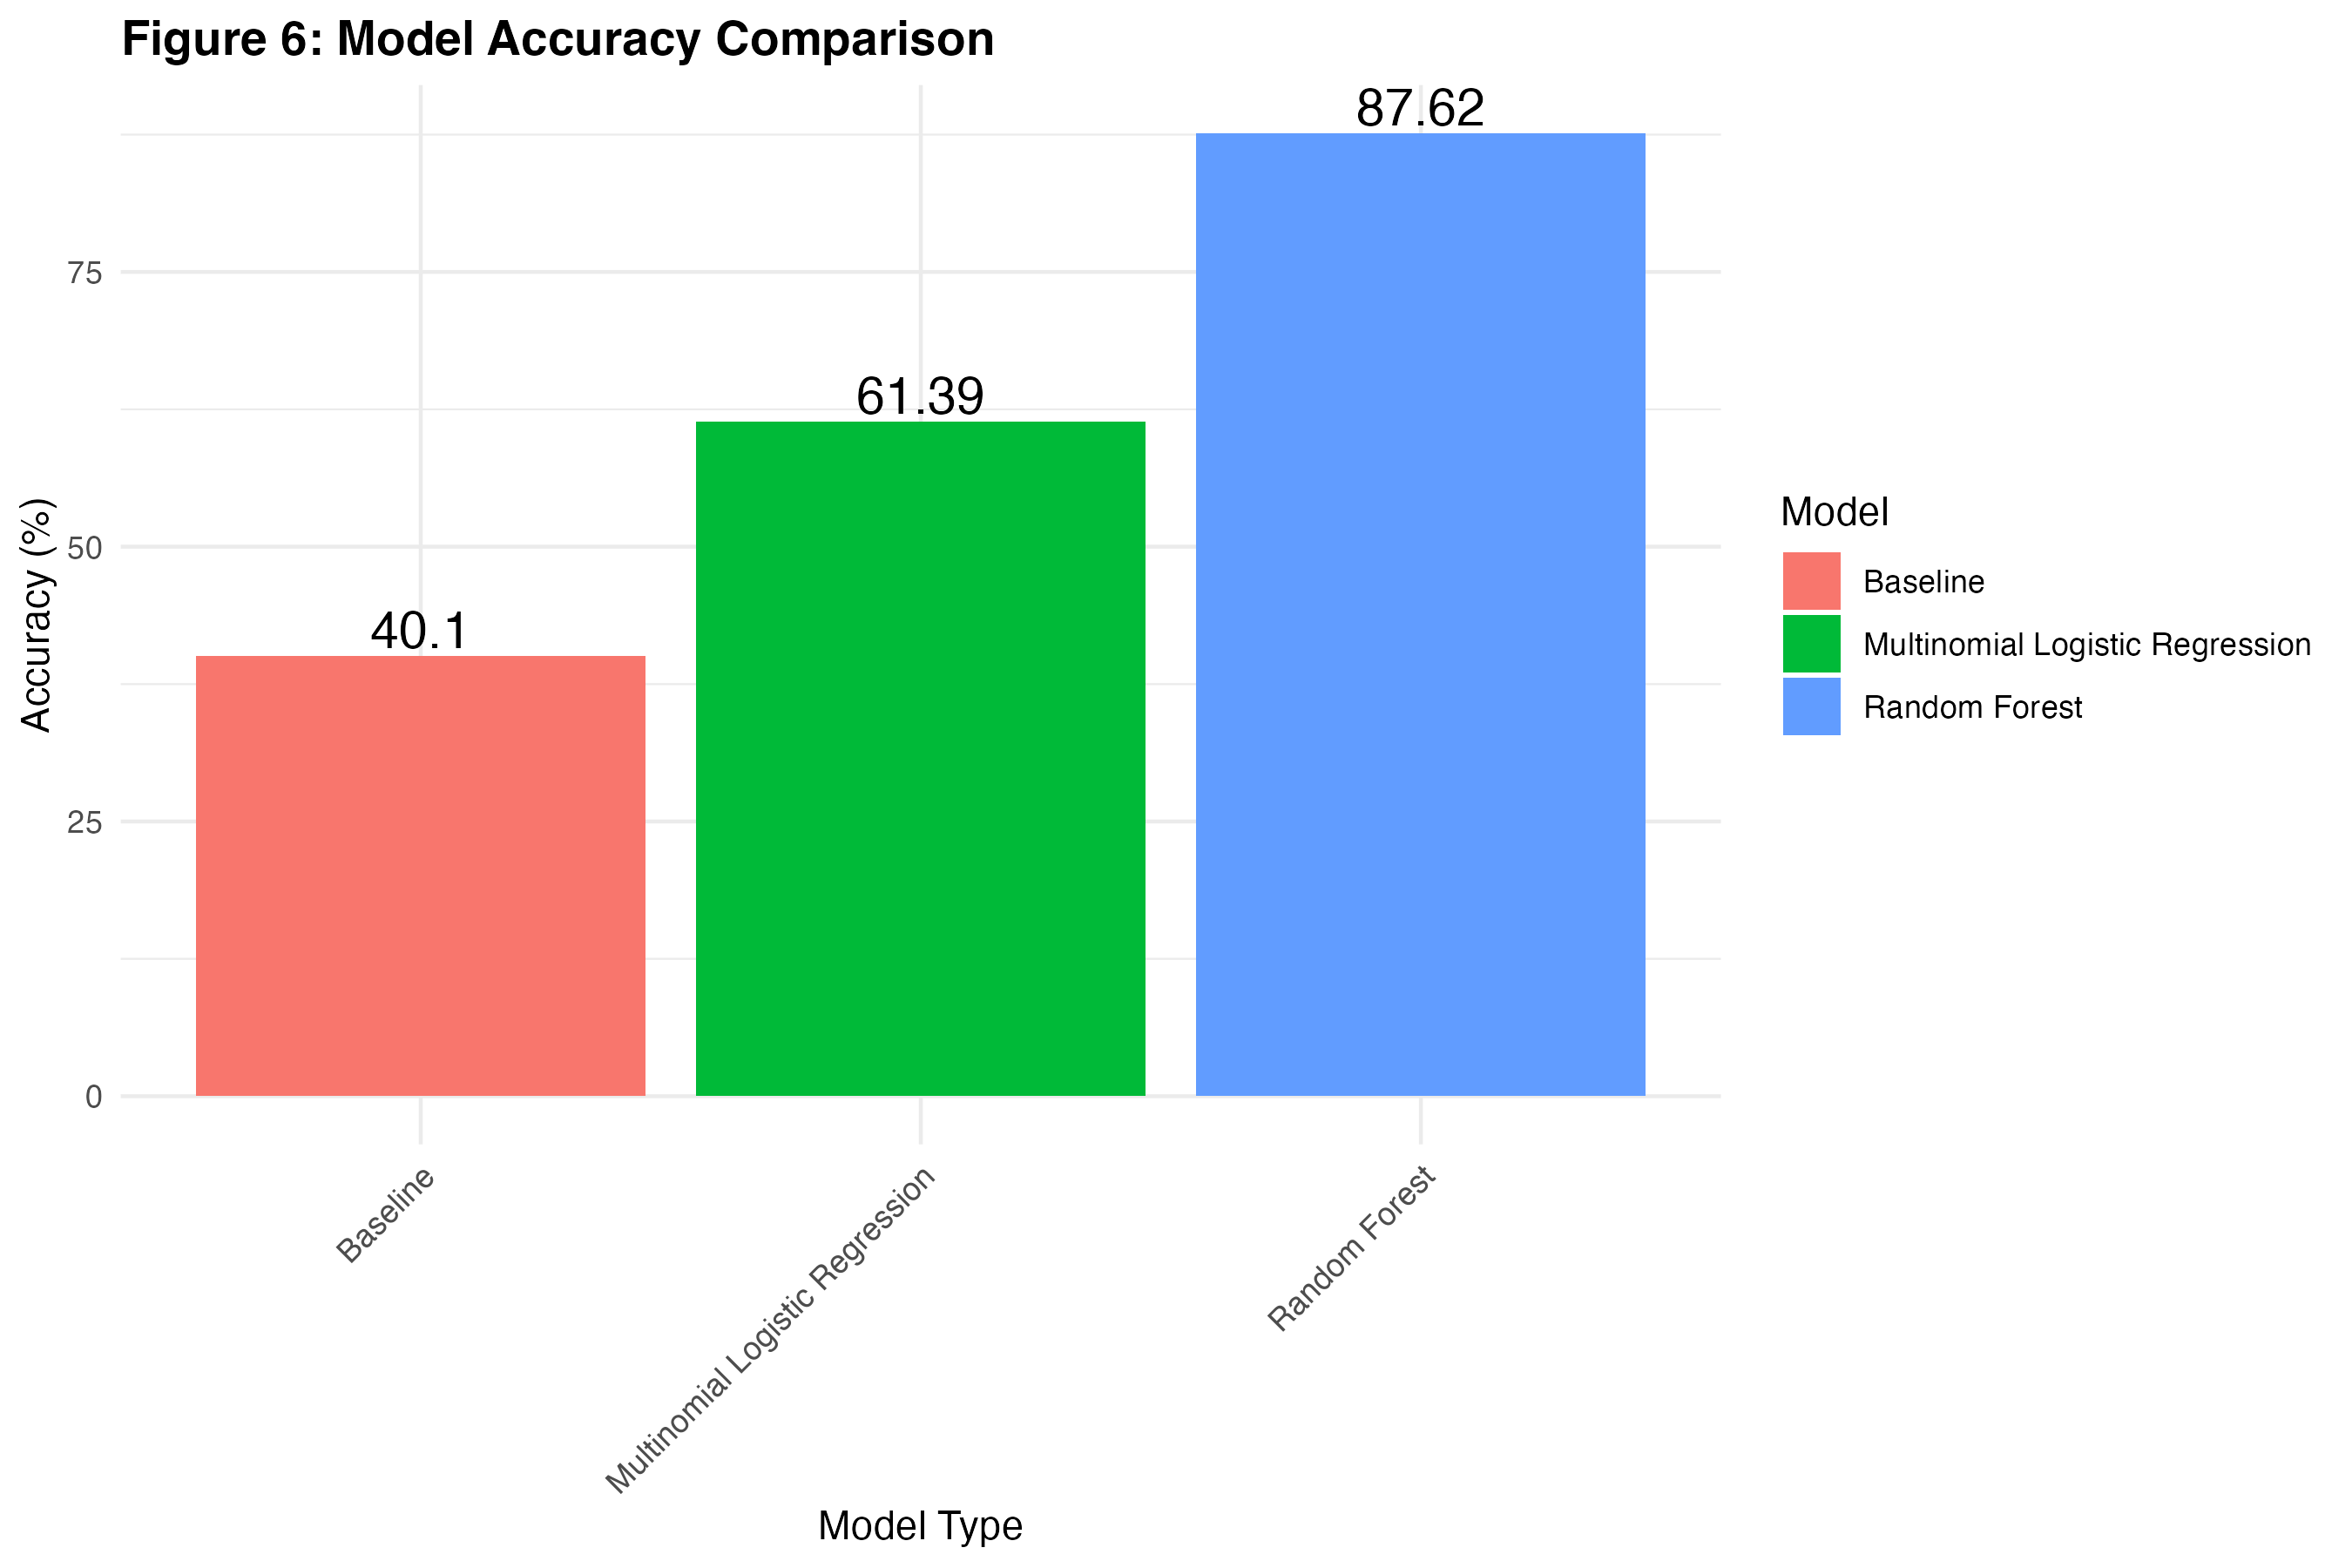
\includegraphics[width=0.8\textwidth,height=\textheight]{../outputs/images/accuracy_comparison.png}

}

\caption{\label{fig-accuracy-comparison}ML Model Accuracies (\%)}

\end{figure}%

From Figure~\ref{fig-accuracy-comparison}, random forest has yielded a
0.8811881 accuracy score, which is 0.2673267 higher than the multinomial
logistic regression accuracy score and 0.480198 higher than of the
baseline model.

\section{Discussion}\label{discussion}

\subsection{Best performing model}\label{best-performing-model}

As shown in the bar graph above, our analyses suggest that maternal
health risk during pregnancy can be predicted with up to a 88.12\%
accuracy using our random forests decision trees model. The second best
model was the multinomial logistic regression that had a 61.39\%
accuracy. Both models performed better than the baseline (40.1\%). Both
models performing better than the baseline is expected as well as the
random forest performing better than the logistic regression as past
literature have found similar results (Mu, Yan, and Zhu 2023; Ukrit et
al. 2024).

\subsection{Interpretation}\label{interpretation}

The multinomial logistic regression, while less accurate, is more
interpretable and gives us an idea of how a 1-unit increase in a
variable is associated with a change in the odds of being in a certain
risk category. For example, the multinomial logistic regression suggests
that a 1 unit increase in Blood Sugar level is associated with an
increase in the odds of being in \texttt{high\ risk} compared to
\texttt{low\ risk} by a factor of 2.1974809.

The best predictors for \texttt{high\ risk} compared to
\texttt{low\ risk} were body temperature (\(OR\) = 2.1442957, \(p\)
\textless{} .001) and blood sugar (\(OR\) = 2.1974809, \(p\) \textless{}
.001). A one unit increase in both was associated with a more than
double increase in the odds of being in the \texttt{high\ risk}
category.

The best predictors for \texttt{medium\ risk} compared to
\texttt{low\ risk} were also body temperature (\(OR\) = 1.4898473, \(p\)
\textless{} .001) and blood sugar (\(OR\) = 1.4546199, \(p\) \textless{}
.001).

Both the multinomial logistic regression model and the Random Forest
model performed best when predicting \texttt{high\ risk}.

\subsection{Impact}\label{impact}

Our analyses show that body temperature and blood sugar are both
relatively strongly associated with increasing maternal health risk. We
do however acknowledge that our models do not necessarily imply a causal
effect such that reducing blood sugar or body temperature will reduce
your maternal health risk. Additionally, our models are limited by the
number of variables we accounted for. Other factors such as age,
parental health conditions, and many more would improve the
generalizability of our models.

Our analyses should therefore not be used as guidelines for pregnant
mothers. Now that we have have further evidence that blood sugar and
body temperature are associated with maternal health risk, future
research could explore the potential causal mechanism of these
relationships. Future research may also explore whether this effect
remains constant across age or whether certain age groups are more
susceptible to the effects of blood sugar/body temperature on maternal
health risk.

\section{References}\label{references}

\phantomsection\label{refs}
\begin{CSLReferences}{1}{0}
\bibitem[\citeproctext]{ref-dataset}
Ahmed, Marzia. 2020. {``{Maternal Health Risk}.''} UCI Machine Learning
Repository.

\bibitem[\citeproctext]{ref-Bajaj-2023}
Bajaj, Disha, Ritika Kumari, and Poonam Bansal. 2023. {``Risk Level
Prediction for Maternal Health Using Machine Learning Algorithms.''}
\emph{2023 International Conference on Communication, Security and
Artificial Intelligence (ICCSAI)}, November, 405--9.
\url{https://doi.org/10.1109/iccsai59793.2023.10421156}.

\bibitem[\citeproctext]{ref-Mu-2023}
Mu, Chenyu, Zexuan Yan, and Yidi Zhu. 2023. {``Prediction of Maternal
Health Risk Based on Physiological Indicators.''} \emph{Proceedings of
the 2023 4th International Symposium on Artificial Intelligence for
Medicine Science}, October, 578--84.
\url{https://doi.org/10.1145/3644116.3644212}.

\bibitem[\citeproctext]{ref-Ukrit-2024}
Ukrit, M.Ferni, R. Beaulah Jeyavathana, Aluru Leela Rani, and Vasa
Chandana. 2024. {``Maternal Health Risk Prediction with Machine Learning
Methods.''} \emph{2024 Second International Conference on Emerging
Trends in Information Technology and Engineering (ICETITE)}, February,
1--9. \url{https://doi.org/10.1109/ic-etite58242.2024.10493737}.

\bibitem[\citeproctext]{ref-who-2024}
WHO. 2024. {``Maternal Mortality Fact Sheet.''} World Health
Organization.
\url{https://www.who.int/news-room/fact-sheets/detail/maternal-mortality}.

\bibitem[\citeproctext]{ref-who-2025}
---------. 2025. {``Maternal Health.''} World Health Organization.
\url{https://www.who.int/health-topics/maternal-health\#tab=tab_1}.

\end{CSLReferences}




\end{document}
